\documentclass[11pt]{article}

\author{Math 123}
\date{Due February 24, 2023 by 5pm} 
\title{Homework 4}

\usepackage{graphicx,xypic}
\usepackage{amsthm}
\usepackage{amsmath,amssymb}
\usepackage{amsfonts}
\usepackage{xcolor}
\usepackage[margin=1in]{geometry}
\usepackage[shortlabels]{enumitem}
\newtheorem{problem}{Problem}
\renewcommand*{\proofname}{{\color{blue}Solution}}


\usepackage{fancyhdr}
\pagestyle{fancy}
\rhead{Math 123, Homework 4}

\setlength{\parindent}{0pt}
\setlength{\parskip}{1.25ex}

% tikz
\usepackage{tikz}
\usetikzlibrary{intersections, angles, quotes, positioning}
\usetikzlibrary{arrows.meta}
\usepackage{pgfplots}
\pgfplotsset{compat=1.13}


\tikzset{
	force/.style={thick, {Circle[length=2pt]}-stealth, shorten <=-1pt}
}

% quiver style
\usepackage{tikz-cd}
% `calc` is necessary to draw curved arrows.
\usetikzlibrary{calc}
% `pathmorphing` is necessary to draw squiggly arrows.
\usetikzlibrary{decorations.pathmorphing}

% A TikZ style for curved arrows of a fixed height, due to AndréC.
\tikzset{curve/.style={settings={#1},to path={(\tikztostart)
					.. controls ($(\tikztostart)!\pv{pos}!(\tikztotarget)!\pv{height}!270:(\tikztotarget)$)
					and ($(\tikztostart)!1-\pv{pos}!(\tikztotarget)!\pv{height}!270:(\tikztotarget)$)
					.. (\tikztotarget)\tikztonodes}},
	settings/.code={\tikzset{quiver/.cd,#1}
			\def\pv##1{\pgfkeysvalueof{/tikz/quiver/##1}}},
	quiver/.cd,pos/.initial=0.35,height/.initial=0}

% TikZ arrowhead/tail styles.
\tikzset{tail reversed/.code={\pgfsetarrowsstart{tikzcd to}}}
\tikzset{2tail/.code={\pgfsetarrowsstart{Implies[reversed]}}}
\tikzset{2tail reversed/.code={\pgfsetarrowsstart{Implies}}}
% TikZ arrow styles.
\tikzset{no body/.style={/tikz/dash pattern=on 0 off 1mm}}

\begin{document}

\maketitle

% You are required to put your name here:
{\bf\Large Name: George Chemmala} 


\vspace{.3in}
Topics covered: matchings, Hall's theorem, maximum matchings, K\"onig's theorem

Instructions: 
\begin{itemize}
\item This assignment must be submitted on Gradescope by the due date. 
\item If you collaborate with other students (which is encouraged!), please mention this near the corresponding problems. 
\item Some problems from this assignment come from West's book, as indicated next to the problem. In some cases, the statements on this assignment differ slightly from the book. 
\item If you are stuck please ask for help (from me or your classmates). Occasionally problems may require ingredients not discussed in the course. 
\item You may freely use any fact proved in class. In general, you should provide proof for facts used that were not proved in class. 
\end{itemize}

\pagebreak 



\begin{problem}
Find a maximum matching in each graph below. Prove that it is a maximum matching by exhibiting an optimal solution to the dual problem. 
\begin{center}
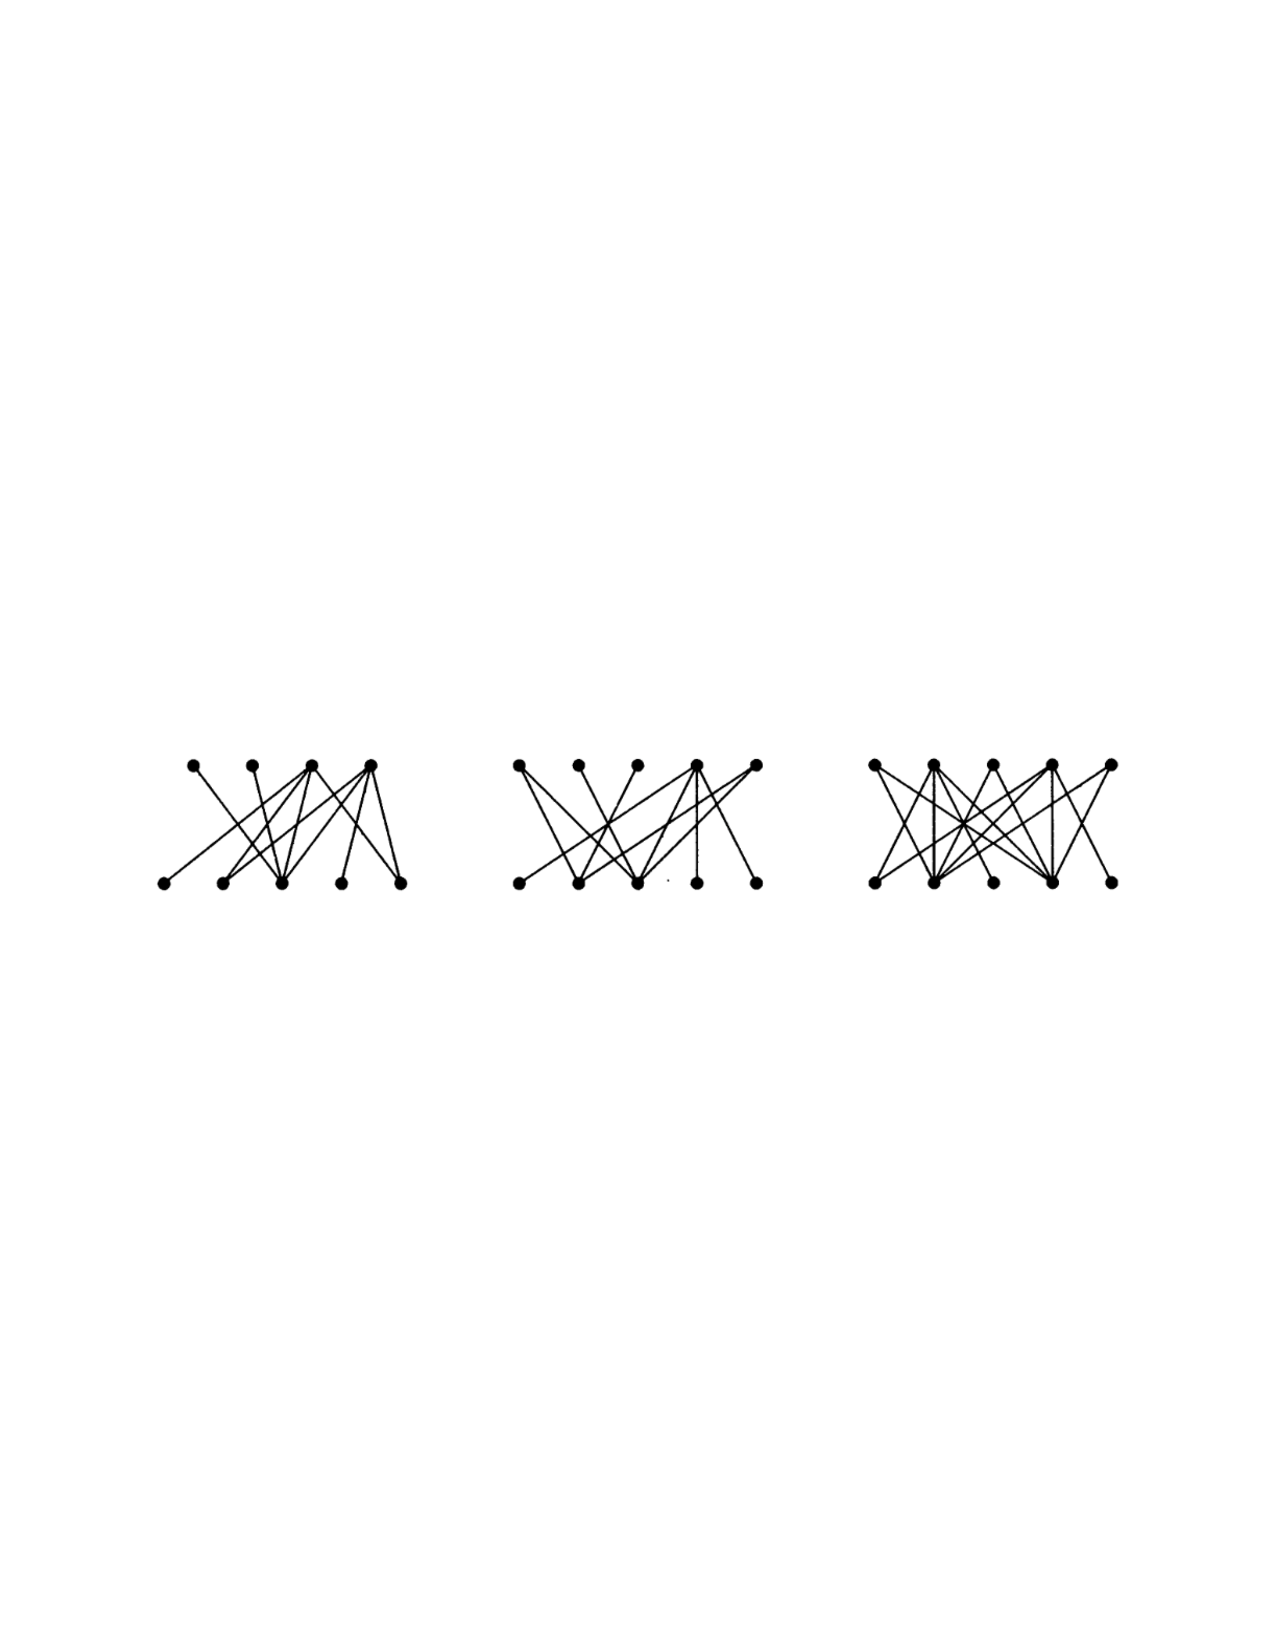
\includegraphics[scale=.8]{matchings.pdf}
\end{center}
\end{problem}

\begin{proof}
\begin{enumerate}
	\item[]
	\item[(a)]
	A matching is created with 3 (dotted) edges
	% https://q.uiver.app/?q=WzAsOSxbMCwwLCJcXGJ1bGxldCJdLFsyLDIsIlxcYnVsbGV0Il0sWzAsMiwiXFxidWxsZXQiXSxbMSwyLCJcXGJ1bGxldCJdLFszLDIsIlxcYnVsbGV0Il0sWzEsMCwiXFxidWxsZXQiXSxbMiwwLCJcXGJ1bGxldCJdLFszLDAsIlxcYnVsbGV0Il0sWzQsMiwiXFxidWxsZXQiXSxbMCwxLCIiLDAseyJzdHlsZSI6eyJib2R5Ijp7Im5hbWUiOiJkYXNoZWQifSwiaGVhZCI6eyJuYW1lIjoibm9uZSJ9fX1dLFs1LDEsIiIsMix7InN0eWxlIjp7ImhlYWQiOnsibmFtZSI6Im5vbmUifX19XSxbNiwxLCIiLDIseyJzdHlsZSI6eyJoZWFkIjp7Im5hbWUiOiJub25lIn19fV0sWzEsNywiIiwyLHsic3R5bGUiOnsiaGVhZCI6eyJuYW1lIjoibm9uZSJ9fX1dLFs3LDQsIiIsMix7InN0eWxlIjp7ImJvZHkiOnsibmFtZSI6ImRhc2hlZCJ9LCJoZWFkIjp7Im5hbWUiOiJub25lIn19fV0sWzcsOCwiIiwyLHsic3R5bGUiOnsiaGVhZCI6eyJuYW1lIjoibm9uZSJ9fX1dLFs4LDYsIiIsMix7InN0eWxlIjp7ImhlYWQiOnsibmFtZSI6Im5vbmUifX19XSxbNiwyLCIiLDIseyJzdHlsZSI6eyJib2R5Ijp7Im5hbWUiOiJkYXNoZWQifSwiaGVhZCI6eyJuYW1lIjoibm9uZSJ9fX1dLFs2LDMsIiIsMix7InN0eWxlIjp7ImhlYWQiOnsibmFtZSI6Im5vbmUifX19XSxbMyw3LCIiLDIseyJzdHlsZSI6eyJoZWFkIjp7Im5hbWUiOiJub25lIn19fV1d
	\[\begin{tikzcd}
		\bullet & \bullet & \bullet & \bullet \\
		\\
		\bullet & \bullet & \bullet & \bullet & \bullet
		\arrow[dashed, no head, from=1-1, to=3-3]
		\arrow[no head, from=1-2, to=3-3]
		\arrow[no head, from=1-3, to=3-3]
		\arrow[no head, from=3-3, to=1-4]
		\arrow[dashed, no head, from=1-4, to=3-4]
		\arrow[no head, from=1-4, to=3-5]
		\arrow[no head, from=3-5, to=1-3]
		\arrow[dashed, no head, from=1-3, to=3-1]
		\arrow[no head, from=1-3, to=3-2]
		\arrow[no head, from=3-2, to=1-4]
	\end{tikzcd}\]
	
	A vertex cover is created using 3 vertices (labeled \(c\) ):
	% https://q.uiver.app/?q=WzAsOSxbMCwwLCJcXGJ1bGxldCJdLFsyLDIsImMiXSxbMCwyLCJcXGJ1bGxldCJdLFsxLDIsIlxcYnVsbGV0Il0sWzMsMiwiXFxidWxsZXQiXSxbMSwwLCJcXGJ1bGxldCJdLFsyLDAsImMiXSxbMywwLCJjIl0sWzQsMiwiXFxidWxsZXQiXSxbMCwxLCIiLDAseyJzdHlsZSI6eyJoZWFkIjp7Im5hbWUiOiJub25lIn19fV0sWzUsMSwiIiwyLHsic3R5bGUiOnsiaGVhZCI6eyJuYW1lIjoibm9uZSJ9fX1dLFs2LDEsIiIsMix7InN0eWxlIjp7ImhlYWQiOnsibmFtZSI6Im5vbmUifX19XSxbMSw3LCIiLDIseyJzdHlsZSI6eyJoZWFkIjp7Im5hbWUiOiJub25lIn19fV0sWzcsNCwiIiwyLHsic3R5bGUiOnsiaGVhZCI6eyJuYW1lIjoibm9uZSJ9fX1dLFs3LDgsIiIsMix7InN0eWxlIjp7ImhlYWQiOnsibmFtZSI6Im5vbmUifX19XSxbOCw2LCIiLDIseyJzdHlsZSI6eyJoZWFkIjp7Im5hbWUiOiJub25lIn19fV0sWzYsMiwiIiwyLHsic3R5bGUiOnsiaGVhZCI6eyJuYW1lIjoibm9uZSJ9fX1dLFs2LDMsIiIsMix7InN0eWxlIjp7ImhlYWQiOnsibmFtZSI6Im5vbmUifX19XSxbMyw3LCIiLDIseyJzdHlsZSI6eyJoZWFkIjp7Im5hbWUiOiJub25lIn19fV1d
	\[\begin{tikzcd}
		\bullet & \bullet & c & c \\
		\\
		\bullet & \bullet & c & \bullet & \bullet
		\arrow[no head, from=1-1, to=3-3]
		\arrow[no head, from=1-2, to=3-3]
		\arrow[no head, from=1-3, to=3-3]
		\arrow[no head, from=3-3, to=1-4]
		\arrow[no head, from=1-4, to=3-4]
		\arrow[no head, from=1-4, to=3-5]
		\arrow[no head, from=3-5, to=1-3]
		\arrow[no head, from=1-3, to=3-1]
		\arrow[no head, from=1-3, to=3-2]
		\arrow[no head, from=3-2, to=1-4]
	\end{tikzcd}\]
	
	Therefore, the previous matching was a maximium matching

	\item[(b)]
	A matching is created with 3 (dotted) edges
	% https://q.uiver.app/?q=WzAsMTAsWzAsMCwiXFxidWxsZXQiXSxbMSwwLCJcXGJ1bGxldCJdLFsyLDAsIlxcYnVsbGV0Il0sWzMsMCwiXFxidWxsZXQiXSxbNCwwLCJcXGJ1bGxldCJdLFswLDIsIlxcYnVsbGV0Il0sWzEsMiwiXFxidWxsZXQiXSxbMiwyLCJcXGJ1bGxldCJdLFszLDIsIlxcYnVsbGV0Il0sWzQsMiwiXFxidWxsZXQiXSxbOSwzLCIiLDAseyJzdHlsZSI6eyJoZWFkIjp7Im5hbWUiOiJub25lIn19fV0sWzMsOCwiIiwwLHsic3R5bGUiOnsiaGVhZCI6eyJuYW1lIjoibm9uZSJ9fX1dLFszLDcsIiIsMCx7InN0eWxlIjp7ImhlYWQiOnsibmFtZSI6Im5vbmUifX19XSxbMyw1LCIiLDAseyJzdHlsZSI6eyJib2R5Ijp7Im5hbWUiOiJkYXNoZWQifSwiaGVhZCI6eyJuYW1lIjoibm9uZSJ9fX1dLFswLDYsIiIsMCx7InN0eWxlIjp7ImJvZHkiOnsibmFtZSI6ImRhc2hlZCJ9LCJoZWFkIjp7Im5hbWUiOiJub25lIn19fV0sWzAsNywiIiwyLHsic3R5bGUiOnsiaGVhZCI6eyJuYW1lIjoibm9uZSJ9fX1dLFsyLDYsIiIsMix7InN0eWxlIjp7ImhlYWQiOnsibmFtZSI6Im5vbmUifX19XSxbMSw3LCIiLDIseyJzdHlsZSI6eyJib2R5Ijp7Im5hbWUiOiJkYXNoZWQifSwiaGVhZCI6eyJuYW1lIjoibm9uZSJ9fX1dLFs3LDQsIiIsMix7InN0eWxlIjp7ImhlYWQiOnsibmFtZSI6Im5vbmUifX19XSxbNiw0LCIiLDIseyJzdHlsZSI6eyJoZWFkIjp7Im5hbWUiOiJub25lIn19fV1d
\[\begin{tikzcd}
	\bullet & \bullet & \bullet & \bullet & \bullet \\
	\\
	\bullet & \bullet & \bullet & \bullet & \bullet
	\arrow[no head, from=3-5, to=1-4]
	\arrow[no head, from=1-4, to=3-4]
	\arrow[no head, from=1-4, to=3-3]
	\arrow[dashed, no head, from=1-4, to=3-1]
	\arrow[dashed, no head, from=1-1, to=3-2]
	\arrow[no head, from=1-1, to=3-3]
	\arrow[no head, from=1-3, to=3-2]
	\arrow[dashed, no head, from=1-2, to=3-3]
	\arrow[no head, from=3-3, to=1-5]
	\arrow[no head, from=3-2, to=1-5]
\end{tikzcd}\]
	
	A vertex cover is created using 3 vertices (labeled \(c\) ):
	% https://q.uiver.app/?q=WzAsMTAsWzAsMCwiXFxidWxsZXQiXSxbMSwwLCJcXGJ1bGxldCJdLFsyLDAsIlxcYnVsbGV0Il0sWzMsMCwiYyJdLFs0LDAsIlxcYnVsbGV0Il0sWzAsMiwiXFxidWxsZXQiXSxbMSwyLCJjIl0sWzIsMiwiYyJdLFszLDIsIlxcYnVsbGV0Il0sWzQsMiwiXFxidWxsZXQiXSxbOSwzLCIiLDAseyJzdHlsZSI6eyJoZWFkIjp7Im5hbWUiOiJub25lIn19fV0sWzMsOCwiIiwwLHsic3R5bGUiOnsiaGVhZCI6eyJuYW1lIjoibm9uZSJ9fX1dLFszLDcsIiIsMCx7InN0eWxlIjp7ImhlYWQiOnsibmFtZSI6Im5vbmUifX19XSxbMyw1LCIiLDAseyJzdHlsZSI6eyJoZWFkIjp7Im5hbWUiOiJub25lIn19fV0sWzAsNiwiIiwwLHsic3R5bGUiOnsiaGVhZCI6eyJuYW1lIjoibm9uZSJ9fX1dLFswLDcsIiIsMix7InN0eWxlIjp7ImhlYWQiOnsibmFtZSI6Im5vbmUifX19XSxbMiw2LCIiLDIseyJzdHlsZSI6eyJoZWFkIjp7Im5hbWUiOiJub25lIn19fV0sWzEsNywiIiwyLHsic3R5bGUiOnsiaGVhZCI6eyJuYW1lIjoibm9uZSJ9fX1dLFs3LDQsIiIsMix7InN0eWxlIjp7ImhlYWQiOnsibmFtZSI6Im5vbmUifX19XSxbNiw0LCIiLDIseyJzdHlsZSI6eyJoZWFkIjp7Im5hbWUiOiJub25lIn19fV1d
\[\begin{tikzcd}
	\bullet & \bullet & \bullet & c & \bullet \\
	\\
	\bullet & c & c & \bullet & \bullet
	\arrow[no head, from=3-5, to=1-4]
	\arrow[no head, from=1-4, to=3-4]
	\arrow[no head, from=1-4, to=3-3]
	\arrow[no head, from=1-4, to=3-1]
	\arrow[no head, from=1-1, to=3-2]
	\arrow[no head, from=1-1, to=3-3]
	\arrow[no head, from=1-3, to=3-2]
	\arrow[no head, from=1-2, to=3-3]
	\arrow[no head, from=3-3, to=1-5]
	\arrow[no head, from=3-2, to=1-5]
\end{tikzcd}\]

	Therefore, the previous matching was a maximium matching

	\item[(c)]
	A matching is created with 4 (dotted) edges
	% https://q.uiver.app/?q=WzAsMTAsWzAsMCwiXFxidWxsZXQiXSxbMSwwLCJcXGJ1bGxldCJdLFsyLDAsIlxcYnVsbGV0Il0sWzMsMCwiXFxidWxsZXQiXSxbNCwwLCJcXGJ1bGxldCJdLFswLDIsIlxcYnVsbGV0Il0sWzEsMiwiXFxidWxsZXQiXSxbMiwyLCJcXGJ1bGxldCJdLFszLDIsIlxcYnVsbGV0Il0sWzQsMiwiXFxidWxsZXQiXSxbNSwxLCIiLDIseyJzdHlsZSI6eyJoZWFkIjp7Im5hbWUiOiJub25lIn19fV0sWzUsMywiIiwwLHsic3R5bGUiOnsiaGVhZCI6eyJuYW1lIjoibm9uZSJ9fX1dLFs2LDAsIiIsMCx7InN0eWxlIjp7ImJvZHkiOnsibmFtZSI6ImRhc2hlZCJ9LCJoZWFkIjp7Im5hbWUiOiJub25lIn19fV0sWzYsMSwiIiwxLHsic3R5bGUiOnsiaGVhZCI6eyJuYW1lIjoibm9uZSJ9fX1dLFs2LDIsIiIsMSx7InN0eWxlIjp7ImhlYWQiOnsibmFtZSI6Im5vbmUifX19XSxbNiwzLCIiLDEseyJzdHlsZSI6eyJoZWFkIjp7Im5hbWUiOiJub25lIn19fV0sWzYsNCwiIiwxLHsic3R5bGUiOnsiaGVhZCI6eyJuYW1lIjoibm9uZSJ9fX1dLFs3LDEsIiIsMSx7InN0eWxlIjp7ImJvZHkiOnsibmFtZSI6ImRhc2hlZCJ9LCJoZWFkIjp7Im5hbWUiOiJub25lIn19fV0sWzgsMCwiIiwyLHsic3R5bGUiOnsiaGVhZCI6eyJuYW1lIjoibm9uZSJ9fX1dLFs4LDEsIiIsMix7InN0eWxlIjp7ImhlYWQiOnsibmFtZSI6Im5vbmUifX19XSxbOCwyLCIiLDIseyJzdHlsZSI6eyJib2R5Ijp7Im5hbWUiOiJkYXNoZWQifSwiaGVhZCI6eyJuYW1lIjoibm9uZSJ9fX1dLFs4LDMsIiIsMix7InN0eWxlIjp7ImhlYWQiOnsibmFtZSI6Im5vbmUifX19XSxbOCw0LCIiLDIseyJzdHlsZSI6eyJoZWFkIjp7Im5hbWUiOiJub25lIn19fV0sWzksMywiIiwyLHsic3R5bGUiOnsiYm9keSI6eyJuYW1lIjoiZGFzaGVkIn0sImhlYWQiOnsibmFtZSI6Im5vbmUifX19XV0=
\[\begin{tikzcd}
	\bullet & \bullet & \bullet & \bullet & \bullet \\
	\\
	\bullet & \bullet & \bullet & \bullet & \bullet
	\arrow[no head, from=3-1, to=1-2]
	\arrow[no head, from=3-1, to=1-4]
	\arrow[dashed, no head, from=3-2, to=1-1]
	\arrow[no head, from=3-2, to=1-2]
	\arrow[no head, from=3-2, to=1-3]
	\arrow[no head, from=3-2, to=1-4]
	\arrow[no head, from=3-2, to=1-5]
	\arrow[dashed, no head, from=3-3, to=1-2]
	\arrow[no head, from=3-4, to=1-1]
	\arrow[no head, from=3-4, to=1-2]
	\arrow[dashed, no head, from=3-4, to=1-3]
	\arrow[no head, from=3-4, to=1-4]
	\arrow[no head, from=3-4, to=1-5]
	\arrow[dashed, no head, from=3-5, to=1-4]
\end{tikzcd}\]

	A vertex cover is created using 4 vertices (labeled \(c\) ):
	% https://q.uiver.app/?q=WzAsMTAsWzAsMCwiXFxidWxsZXQiXSxbMSwwLCJjIl0sWzIsMCwiXFxidWxsZXQiXSxbMywwLCJjIl0sWzQsMCwiXFxidWxsZXQiXSxbMCwyLCJcXGJ1bGxldCJdLFsxLDIsImMiXSxbMiwyLCJcXGJ1bGxldCJdLFszLDIsImMiXSxbNCwyLCJcXGJ1bGxldCJdLFswLDYsIiIsMCx7InN0eWxlIjp7ImhlYWQiOnsibmFtZSI6Im5vbmUifX19XSxbMSw2LCIiLDIseyJzdHlsZSI6eyJoZWFkIjp7Im5hbWUiOiJub25lIn19fV0sWzIsNiwiIiwyLHsic3R5bGUiOnsiaGVhZCI6eyJuYW1lIjoibm9uZSJ9fX1dLFszLDYsIiIsMix7InN0eWxlIjp7ImhlYWQiOnsibmFtZSI6Im5vbmUifX19XSxbNCw2LCIiLDIseyJzdHlsZSI6eyJoZWFkIjp7Im5hbWUiOiJub25lIn19fV0sWzUsMSwiIiwyLHsic3R5bGUiOnsiaGVhZCI6eyJuYW1lIjoibm9uZSJ9fX1dLFs1LDMsIiIsMSx7InN0eWxlIjp7ImhlYWQiOnsibmFtZSI6Im5vbmUifX19XSxbNywxLCIiLDEseyJzdHlsZSI6eyJoZWFkIjp7Im5hbWUiOiJub25lIn19fV0sWzgsMCwiIiwwLHsic3R5bGUiOnsiaGVhZCI6eyJuYW1lIjoibm9uZSJ9fX1dLFs4LDEsIiIsMCx7InN0eWxlIjp7ImhlYWQiOnsibmFtZSI6Im5vbmUifX19XSxbOCwzLCIiLDAseyJzdHlsZSI6eyJoZWFkIjp7Im5hbWUiOiJub25lIn19fV0sWzgsNCwiIiwyLHsic3R5bGUiOnsiaGVhZCI6eyJuYW1lIjoibm9uZSJ9fX1dLFs5LDMsIiIsMix7InN0eWxlIjp7ImhlYWQiOnsibmFtZSI6Im5vbmUifX19XSxbOCwyXV0=
\[\begin{tikzcd}
	\bullet & c & \bullet & c & \bullet \\
	\\
	\bullet & c & \bullet & c & \bullet
	\arrow[no head, from=1-1, to=3-2]
	\arrow[no head, from=1-2, to=3-2]
	\arrow[no head, from=1-3, to=3-2]
	\arrow[no head, from=1-4, to=3-2]
	\arrow[no head, from=1-5, to=3-2]
	\arrow[no head, from=3-1, to=1-2]
	\arrow[no head, from=3-1, to=1-4]
	\arrow[no head, from=3-3, to=1-2]
	\arrow[no head, from=3-4, to=1-1]
	\arrow[no head, from=3-4, to=1-2]
	\arrow[no head, from=3-4, to=1-4]
	\arrow[no head, from=3-4, to=1-5]
	\arrow[no head, from=3-5, to=1-4]
	\arrow[from=3-4, to=1-3]
\end{tikzcd}\]

	Therefore, the previous matching was a maximium matching
\end{enumerate}

The matchings and their equivalent vertex covers share the same size; therefore, the matchings are maximum, and the covers are minimums.
\end{proof}



\begin{problem}
Prove or disprove: every tree $T$ has at most one perfect matching. 
\end{problem}

\begin{proof}
Let \(M\) and \(N\) be two perfect matchings of \(T\). When we take the symmetric difference (\(M \triangle N\)) we find that every vertex has degree \(0\) or \(2\) (shown in class). Therefore, (\(M \triangle N\)) contains independent vertices (from \(0\) degree vertices) and cycles from the \(2\) degree vertices (2-regular components are cycles). The matchings \(M\) and \(N\) are subgraphs of \(T\), and (\(M \triangle N\)) is a subgraph of \(M \cup N\), so \(M \triangle N\) is a subgraph of \(T\) and thus has no cycles. Therefore, all vertices in \(M \triangle N\) must have degree \(0\) and therefore, the edges in \(M\) and \(N\) are the same since if they weren't, an edge unique to one of \(M\) or \(N\) would be in \(M \triangle N\). 
\end{proof}


\begin{problem}
Construct a $3$-regular graph with an even number of vertices and no perfect matching. Give proof that your graph has the desired property. 
\end{problem}

\begin{proof}
Graph:
% https://q.uiver.app/?q=WzAsMTYsWzMsMywiXFxidWxsZXQiXSxbNCwzLCJcXGJ1bGxldCJdLFsyLDMsIlxcYnVsbGV0Il0sWzMsMiwiXFxidWxsZXQiXSxbNSwyLCJcXGJ1bGxldCJdLFs2LDMsIlxcYnVsbGV0Il0sWzUsNCwiXFxidWxsZXQiXSxbNSwzLCJcXGJ1bGxldCJdLFsxLDIsIlxcYnVsbGV0Il0sWzAsMywiXFxidWxsZXQiXSxbMSw0LCJcXGJ1bGxldCJdLFsxLDMsIlxcYnVsbGV0Il0sWzQsMSwiXFxidWxsZXQiXSxbMywwLCJcXGJ1bGxldCJdLFsyLDEsIlxcYnVsbGV0Il0sWzMsMSwiXFxidWxsZXQiXSxbMCwxLCIiLDAseyJzdHlsZSI6eyJoZWFkIjp7Im5hbWUiOiJub25lIn19fV0sWzAsMiwiIiwyLHsic3R5bGUiOnsiaGVhZCI6eyJuYW1lIjoibm9uZSJ9fX1dLFswLDMsIiIsMix7InN0eWxlIjp7ImhlYWQiOnsibmFtZSI6Im5vbmUifX19XSxbMSw0LCIiLDAseyJzdHlsZSI6eyJoZWFkIjp7Im5hbWUiOiJub25lIn19fV0sWzQsNSwiIiwwLHsic3R5bGUiOnsiaGVhZCI6eyJuYW1lIjoibm9uZSJ9fX1dLFs1LDYsIiIsMCx7InN0eWxlIjp7ImhlYWQiOnsibmFtZSI6Im5vbmUifX19XSxbNiwxLCIiLDAseyJzdHlsZSI6eyJoZWFkIjp7Im5hbWUiOiJub25lIn19fV0sWzcsNCwiIiwwLHsic3R5bGUiOnsiaGVhZCI6eyJuYW1lIjoibm9uZSJ9fX1dLFs3LDYsIiIsMCx7InN0eWxlIjp7ImhlYWQiOnsibmFtZSI6Im5vbmUifX19XSxbNyw1LCIiLDAseyJzdHlsZSI6eyJoZWFkIjp7Im5hbWUiOiJub25lIn19fV0sWzIsOCwiIiwyLHsic3R5bGUiOnsiaGVhZCI6eyJuYW1lIjoibm9uZSJ9fX1dLFs4LDksIiIsMix7InN0eWxlIjp7ImhlYWQiOnsibmFtZSI6Im5vbmUifX19XSxbOSwxMCwiIiwyLHsic3R5bGUiOnsiaGVhZCI6eyJuYW1lIjoibm9uZSJ9fX1dLFsxMCwyLCIiLDIseyJzdHlsZSI6eyJoZWFkIjp7Im5hbWUiOiJub25lIn19fV0sWzExLDgsIiIsMix7InN0eWxlIjp7ImhlYWQiOnsibmFtZSI6Im5vbmUifX19XSxbMTEsMTAsIiIsMix7InN0eWxlIjp7ImhlYWQiOnsibmFtZSI6Im5vbmUifX19XSxbMTEsOSwiIiwyLHsic3R5bGUiOnsiaGVhZCI6eyJuYW1lIjoibm9uZSJ9fX1dLFszLDEyLCIiLDIseyJzdHlsZSI6eyJoZWFkIjp7Im5hbWUiOiJub25lIn19fV0sWzEyLDEzLCIiLDIseyJzdHlsZSI6eyJoZWFkIjp7Im5hbWUiOiJub25lIn19fV0sWzEzLDE0LCIiLDIseyJzdHlsZSI6eyJoZWFkIjp7Im5hbWUiOiJub25lIn19fV0sWzE0LDMsIiIsMix7InN0eWxlIjp7ImhlYWQiOnsibmFtZSI6Im5vbmUifX19XSxbMTUsMTQsIiIsMix7InN0eWxlIjp7ImhlYWQiOnsibmFtZSI6Im5vbmUifX19XSxbMTUsMTIsIiIsMix7InN0eWxlIjp7ImhlYWQiOnsibmFtZSI6Im5vbmUifX19XSxbMTUsMTMsIiIsMix7InN0eWxlIjp7ImhlYWQiOnsibmFtZSI6Im5vbmUifX19XV0=
\[\begin{tikzcd}
	&&& \bullet \\
	&& \bullet & \bullet & \bullet \\
	& \bullet && \bullet && \bullet \\
	\bullet & \bullet & \bullet & \bullet & \bullet & \bullet & \bullet \\
	& \bullet &&&& \bullet
	\arrow[no head, from=4-4, to=4-5]
	\arrow[no head, from=4-4, to=4-3]
	\arrow[no head, from=4-4, to=3-4]
	\arrow[no head, from=4-5, to=3-6]
	\arrow[no head, from=3-6, to=4-7]
	\arrow[no head, from=4-7, to=5-6]
	\arrow[no head, from=5-6, to=4-5]
	\arrow[no head, from=4-6, to=3-6]
	\arrow[no head, from=4-6, to=5-6]
	\arrow[no head, from=4-6, to=4-7]
	\arrow[no head, from=4-3, to=3-2]
	\arrow[no head, from=3-2, to=4-1]
	\arrow[no head, from=4-1, to=5-2]
	\arrow[no head, from=5-2, to=4-3]
	\arrow[no head, from=4-2, to=3-2]
	\arrow[no head, from=4-2, to=5-2]
	\arrow[no head, from=4-2, to=4-1]
	\arrow[no head, from=3-4, to=2-5]
	\arrow[no head, from=2-5, to=1-4]
	\arrow[no head, from=1-4, to=2-3]
	\arrow[no head, from=2-3, to=3-4]
	\arrow[no head, from=2-4, to=2-3]
	\arrow[no head, from=2-4, to=2-5]
	\arrow[no head, from=2-4, to=1-4]
\end{tikzcd}\]

Proof:
All vertices have degree \(3\) and there are \(16 = 2(8)\) vertices, an even number. 
Let's try to create a perfect matching and show how that leads to a contradiction:

We will begin with a blank (dotted) graph.
% https://q.uiver.app/?q=WzAsMTYsWzMsMywiXFxidWxsZXQiXSxbNCwzLCJcXGJ1bGxldCJdLFsyLDMsIlxcYnVsbGV0Il0sWzMsMiwiXFxidWxsZXQiXSxbNSwyLCJcXGJ1bGxldCJdLFs2LDMsIlxcYnVsbGV0Il0sWzUsNCwiXFxidWxsZXQiXSxbNSwzLCJcXGJ1bGxldCJdLFsxLDIsIlxcYnVsbGV0Il0sWzAsMywiXFxidWxsZXQiXSxbMSw0LCJcXGJ1bGxldCJdLFsxLDMsIlxcYnVsbGV0Il0sWzQsMSwiXFxidWxsZXQiXSxbMywwLCJcXGJ1bGxldCJdLFsyLDEsIlxcYnVsbGV0Il0sWzMsMSwiXFxidWxsZXQiXSxbMCwxLCIiLDAseyJzdHlsZSI6eyJib2R5Ijp7Im5hbWUiOiJkYXNoZWQifSwiaGVhZCI6eyJuYW1lIjoibm9uZSJ9fX1dLFswLDIsIiIsMix7InN0eWxlIjp7ImJvZHkiOnsibmFtZSI6ImRhc2hlZCJ9LCJoZWFkIjp7Im5hbWUiOiJub25lIn19fV0sWzAsMywiIiwyLHsic3R5bGUiOnsiYm9keSI6eyJuYW1lIjoiZGFzaGVkIn0sImhlYWQiOnsibmFtZSI6Im5vbmUifX19XSxbMSw0LCIiLDAseyJzdHlsZSI6eyJib2R5Ijp7Im5hbWUiOiJkYXNoZWQifSwiaGVhZCI6eyJuYW1lIjoibm9uZSJ9fX1dLFs0LDUsIiIsMCx7InN0eWxlIjp7ImJvZHkiOnsibmFtZSI6ImRhc2hlZCJ9LCJoZWFkIjp7Im5hbWUiOiJub25lIn19fV0sWzUsNiwiIiwwLHsic3R5bGUiOnsiYm9keSI6eyJuYW1lIjoiZGFzaGVkIn0sImhlYWQiOnsibmFtZSI6Im5vbmUifX19XSxbNiwxLCIiLDAseyJzdHlsZSI6eyJib2R5Ijp7Im5hbWUiOiJkYXNoZWQifSwiaGVhZCI6eyJuYW1lIjoibm9uZSJ9fX1dLFs3LDQsIiIsMCx7InN0eWxlIjp7ImJvZHkiOnsibmFtZSI6ImRhc2hlZCJ9LCJoZWFkIjp7Im5hbWUiOiJub25lIn19fV0sWzcsNiwiIiwwLHsic3R5bGUiOnsiYm9keSI6eyJuYW1lIjoiZGFzaGVkIn0sImhlYWQiOnsibmFtZSI6Im5vbmUifX19XSxbNyw1LCIiLDAseyJzdHlsZSI6eyJib2R5Ijp7Im5hbWUiOiJkYXNoZWQifSwiaGVhZCI6eyJuYW1lIjoibm9uZSJ9fX1dLFsyLDgsIiIsMix7InN0eWxlIjp7ImJvZHkiOnsibmFtZSI6ImRhc2hlZCJ9LCJoZWFkIjp7Im5hbWUiOiJub25lIn19fV0sWzgsOSwiIiwyLHsic3R5bGUiOnsiYm9keSI6eyJuYW1lIjoiZGFzaGVkIn0sImhlYWQiOnsibmFtZSI6Im5vbmUifX19XSxbOSwxMCwiIiwyLHsic3R5bGUiOnsiYm9keSI6eyJuYW1lIjoiZGFzaGVkIn0sImhlYWQiOnsibmFtZSI6Im5vbmUifX19XSxbMTAsMiwiIiwyLHsic3R5bGUiOnsiYm9keSI6eyJuYW1lIjoiZGFzaGVkIn0sImhlYWQiOnsibmFtZSI6Im5vbmUifX19XSxbMTEsOCwiIiwyLHsic3R5bGUiOnsiYm9keSI6eyJuYW1lIjoiZGFzaGVkIn0sImhlYWQiOnsibmFtZSI6Im5vbmUifX19XSxbMTEsMTAsIiIsMix7InN0eWxlIjp7ImJvZHkiOnsibmFtZSI6ImRhc2hlZCJ9LCJoZWFkIjp7Im5hbWUiOiJub25lIn19fV0sWzExLDksIiIsMix7InN0eWxlIjp7ImJvZHkiOnsibmFtZSI6ImRhc2hlZCJ9LCJoZWFkIjp7Im5hbWUiOiJub25lIn19fV0sWzMsMTIsIiIsMix7InN0eWxlIjp7ImJvZHkiOnsibmFtZSI6ImRhc2hlZCJ9LCJoZWFkIjp7Im5hbWUiOiJub25lIn19fV0sWzEyLDEzLCIiLDIseyJzdHlsZSI6eyJib2R5Ijp7Im5hbWUiOiJkYXNoZWQifSwiaGVhZCI6eyJuYW1lIjoibm9uZSJ9fX1dLFsxMywxNCwiIiwyLHsic3R5bGUiOnsiYm9keSI6eyJuYW1lIjoiZGFzaGVkIn0sImhlYWQiOnsibmFtZSI6Im5vbmUifX19XSxbMTQsMywiIiwyLHsic3R5bGUiOnsiYm9keSI6eyJuYW1lIjoiZGFzaGVkIn0sImhlYWQiOnsibmFtZSI6Im5vbmUifX19XSxbMTUsMTQsIiIsMix7InN0eWxlIjp7ImJvZHkiOnsibmFtZSI6ImRhc2hlZCJ9LCJoZWFkIjp7Im5hbWUiOiJub25lIn19fV0sWzE1LDEyLCIiLDIseyJzdHlsZSI6eyJib2R5Ijp7Im5hbWUiOiJkYXNoZWQifSwiaGVhZCI6eyJuYW1lIjoibm9uZSJ9fX1dLFsxNSwxMywiIiwyLHsic3R5bGUiOnsiYm9keSI6eyJuYW1lIjoiZGFzaGVkIn0sImhlYWQiOnsibmFtZSI6Im5vbmUifX19XV0=
\[\begin{tikzcd}
	&&& \bullet \\
	&& \bullet & \bullet & \bullet \\
	& \bullet && \bullet && \bullet \\
	\bullet & \bullet & \bullet & \bullet & \bullet & \bullet & \bullet \\
	& \bullet &&&& \bullet
	\arrow[dashed, no head, from=4-4, to=4-5]
	\arrow[dashed, no head, from=4-4, to=4-3]
	\arrow[dashed, no head, from=4-4, to=3-4]
	\arrow[dashed, no head, from=4-5, to=3-6]
	\arrow[dashed, no head, from=3-6, to=4-7]
	\arrow[dashed, no head, from=4-7, to=5-6]
	\arrow[dashed, no head, from=5-6, to=4-5]
	\arrow[dashed, no head, from=4-6, to=3-6]
	\arrow[dashed, no head, from=4-6, to=5-6]
	\arrow[dashed, no head, from=4-6, to=4-7]
	\arrow[dashed, no head, from=4-3, to=3-2]
	\arrow[dashed, no head, from=3-2, to=4-1]
	\arrow[dashed, no head, from=4-1, to=5-2]
	\arrow[dashed, no head, from=5-2, to=4-3]
	\arrow[dashed, no head, from=4-2, to=3-2]
	\arrow[dashed, no head, from=4-2, to=5-2]
	\arrow[dashed, no head, from=4-2, to=4-1]
	\arrow[dashed, no head, from=3-4, to=2-5]
	\arrow[dashed, no head, from=2-5, to=1-4]
	\arrow[dashed, no head, from=1-4, to=2-3]
	\arrow[dashed, no head, from=2-3, to=3-4]
	\arrow[dashed, no head, from=2-4, to=2-3]
	\arrow[dashed, no head, from=2-4, to=2-5]
	\arrow[dashed, no head, from=2-4, to=1-4]
\end{tikzcd}\]

We can see that the center vertex, which connects the square shaped subgraphs, has \(3\) edges and thus one of the edges must be part of the matching. Because of the 3-fold symmetry, we can assume without loss of generality that the top edge is part of the matching as seen bellow:
% https://q.uiver.app/?q=WzAsMTYsWzMsMywiXFxidWxsZXQiXSxbNCwzLCJcXGJ1bGxldCJdLFsyLDMsIlxcYnVsbGV0Il0sWzMsMiwiXFxidWxsZXQiXSxbNSwyLCJcXGJ1bGxldCJdLFs2LDMsIlxcYnVsbGV0Il0sWzUsNCwiXFxidWxsZXQiXSxbNSwzLCJcXGJ1bGxldCJdLFsxLDIsIlxcYnVsbGV0Il0sWzAsMywiXFxidWxsZXQiXSxbMSw0LCJcXGJ1bGxldCJdLFsxLDMsIlxcYnVsbGV0Il0sWzQsMSwiXFxidWxsZXQiXSxbMywwLCJcXGJ1bGxldCJdLFsyLDEsIlxcYnVsbGV0Il0sWzMsMSwiXFxidWxsZXQiXSxbMCwxLCIiLDAseyJzdHlsZSI6eyJib2R5Ijp7Im5hbWUiOiJub25lIn0sImhlYWQiOnsibmFtZSI6Im5vbmUifX19XSxbMCwyLCIiLDIseyJzdHlsZSI6eyJib2R5Ijp7Im5hbWUiOiJub25lIn0sImhlYWQiOnsibmFtZSI6Im5vbmUifX19XSxbMCwzLCIiLDIseyJzdHlsZSI6eyJoZWFkIjp7Im5hbWUiOiJub25lIn19fV0sWzEsNCwiIiwwLHsic3R5bGUiOnsiYm9keSI6eyJuYW1lIjoiZGFzaGVkIn0sImhlYWQiOnsibmFtZSI6Im5vbmUifX19XSxbNCw1LCIiLDAseyJzdHlsZSI6eyJib2R5Ijp7Im5hbWUiOiJkYXNoZWQifSwiaGVhZCI6eyJuYW1lIjoibm9uZSJ9fX1dLFs1LDYsIiIsMCx7InN0eWxlIjp7ImJvZHkiOnsibmFtZSI6ImRhc2hlZCJ9LCJoZWFkIjp7Im5hbWUiOiJub25lIn19fV0sWzYsMSwiIiwwLHsic3R5bGUiOnsiYm9keSI6eyJuYW1lIjoiZGFzaGVkIn0sImhlYWQiOnsibmFtZSI6Im5vbmUifX19XSxbNyw0LCIiLDAseyJzdHlsZSI6eyJib2R5Ijp7Im5hbWUiOiJkYXNoZWQifSwiaGVhZCI6eyJuYW1lIjoibm9uZSJ9fX1dLFs3LDYsIiIsMCx7InN0eWxlIjp7ImJvZHkiOnsibmFtZSI6ImRhc2hlZCJ9LCJoZWFkIjp7Im5hbWUiOiJub25lIn19fV0sWzcsNSwiIiwwLHsic3R5bGUiOnsiYm9keSI6eyJuYW1lIjoiZGFzaGVkIn0sImhlYWQiOnsibmFtZSI6Im5vbmUifX19XSxbMiw4LCIiLDIseyJzdHlsZSI6eyJib2R5Ijp7Im5hbWUiOiJkYXNoZWQifSwiaGVhZCI6eyJuYW1lIjoibm9uZSJ9fX1dLFs4LDksIiIsMix7InN0eWxlIjp7ImJvZHkiOnsibmFtZSI6ImRhc2hlZCJ9LCJoZWFkIjp7Im5hbWUiOiJub25lIn19fV0sWzksMTAsIiIsMix7InN0eWxlIjp7ImJvZHkiOnsibmFtZSI6ImRhc2hlZCJ9LCJoZWFkIjp7Im5hbWUiOiJub25lIn19fV0sWzEwLDIsIiIsMix7InN0eWxlIjp7ImJvZHkiOnsibmFtZSI6ImRhc2hlZCJ9LCJoZWFkIjp7Im5hbWUiOiJub25lIn19fV0sWzExLDgsIiIsMix7InN0eWxlIjp7ImJvZHkiOnsibmFtZSI6ImRhc2hlZCJ9LCJoZWFkIjp7Im5hbWUiOiJub25lIn19fV0sWzExLDEwLCIiLDIseyJzdHlsZSI6eyJib2R5Ijp7Im5hbWUiOiJkYXNoZWQifSwiaGVhZCI6eyJuYW1lIjoibm9uZSJ9fX1dLFsxMSw5LCIiLDIseyJzdHlsZSI6eyJib2R5Ijp7Im5hbWUiOiJkYXNoZWQifSwiaGVhZCI6eyJuYW1lIjoibm9uZSJ9fX1dLFszLDEyLCIiLDIseyJzdHlsZSI6eyJib2R5Ijp7Im5hbWUiOiJkYXNoZWQifSwiaGVhZCI6eyJuYW1lIjoibm9uZSJ9fX1dLFsxMiwxMywiIiwyLHsic3R5bGUiOnsiYm9keSI6eyJuYW1lIjoiZGFzaGVkIn0sImhlYWQiOnsibmFtZSI6Im5vbmUifX19XSxbMTMsMTQsIiIsMix7InN0eWxlIjp7ImJvZHkiOnsibmFtZSI6ImRhc2hlZCJ9LCJoZWFkIjp7Im5hbWUiOiJub25lIn19fV0sWzE0LDMsIiIsMix7InN0eWxlIjp7ImJvZHkiOnsibmFtZSI6ImRhc2hlZCJ9LCJoZWFkIjp7Im5hbWUiOiJub25lIn19fV0sWzE1LDE0LCIiLDIseyJzdHlsZSI6eyJib2R5Ijp7Im5hbWUiOiJkYXNoZWQifSwiaGVhZCI6eyJuYW1lIjoibm9uZSJ9fX1dLFsxNSwxMiwiIiwyLHsic3R5bGUiOnsiYm9keSI6eyJuYW1lIjoiZGFzaGVkIn0sImhlYWQiOnsibmFtZSI6Im5vbmUifX19XSxbMTUsMTMsIiIsMix7InN0eWxlIjp7ImJvZHkiOnsibmFtZSI6ImRhc2hlZCJ9LCJoZWFkIjp7Im5hbWUiOiJub25lIn19fV1d
\[\begin{tikzcd}
	&&& \bullet \\
	&& \bullet & \bullet & \bullet \\
	& \bullet && \bullet && \bullet \\
	\bullet & \bullet & \bullet & \bullet & \bullet & \bullet & \bullet \\
	& \bullet &&&& \bullet
	\arrow[draw=none, from=4-4, to=4-5]
	\arrow[draw=none, from=4-4, to=4-3]
	\arrow[no head, from=4-4, to=3-4]
	\arrow[dashed, no head, from=4-5, to=3-6]
	\arrow[dashed, no head, from=3-6, to=4-7]
	\arrow[dashed, no head, from=4-7, to=5-6]
	\arrow[dashed, no head, from=5-6, to=4-5]
	\arrow[dashed, no head, from=4-6, to=3-6]
	\arrow[dashed, no head, from=4-6, to=5-6]
	\arrow[dashed, no head, from=4-6, to=4-7]
	\arrow[dashed, no head, from=4-3, to=3-2]
	\arrow[dashed, no head, from=3-2, to=4-1]
	\arrow[dashed, no head, from=4-1, to=5-2]
	\arrow[dashed, no head, from=5-2, to=4-3]
	\arrow[dashed, no head, from=4-2, to=3-2]
	\arrow[dashed, no head, from=4-2, to=5-2]
	\arrow[dashed, no head, from=4-2, to=4-1]
	\arrow[dashed, no head, from=3-4, to=2-5]
	\arrow[dashed, no head, from=2-5, to=1-4]
	\arrow[dashed, no head, from=1-4, to=2-3]
	\arrow[dashed, no head, from=2-3, to=3-4]
	\arrow[dashed, no head, from=2-4, to=2-3]
	\arrow[dashed, no head, from=2-4, to=2-5]
	\arrow[dashed, no head, from=2-4, to=1-4]
\end{tikzcd}\]

Now we can focus on one of the square shaped subgraphs not attached to the center vertex. Because of the vertical symmetry, we can assume without loss of generality to focus on the subgraph on the right. Because of the horizontal symmetry, we can assume without loss of generality that the left most vertex is connected to the topmost vertex.
% https://q.uiver.app/?q=WzAsMTYsWzMsMywiXFxidWxsZXQiXSxbNCwzLCJcXGJ1bGxldCJdLFsyLDMsIlxcYnVsbGV0Il0sWzMsMiwiXFxidWxsZXQiXSxbNSwyLCJcXGJ1bGxldCJdLFs2LDMsIlxcYnVsbGV0Il0sWzUsNCwiXFxidWxsZXQiXSxbNSwzLCJcXGJ1bGxldCJdLFsxLDIsIlxcYnVsbGV0Il0sWzAsMywiXFxidWxsZXQiXSxbMSw0LCJcXGJ1bGxldCJdLFsxLDMsIlxcYnVsbGV0Il0sWzQsMSwiXFxidWxsZXQiXSxbMywwLCJcXGJ1bGxldCJdLFsyLDEsIlxcYnVsbGV0Il0sWzMsMSwiXFxidWxsZXQiXSxbMCwxLCIiLDAseyJzdHlsZSI6eyJib2R5Ijp7Im5hbWUiOiJub25lIn0sImhlYWQiOnsibmFtZSI6Im5vbmUifX19XSxbMCwyLCIiLDIseyJzdHlsZSI6eyJib2R5Ijp7Im5hbWUiOiJub25lIn0sImhlYWQiOnsibmFtZSI6Im5vbmUifX19XSxbMCwzLCIiLDIseyJzdHlsZSI6eyJoZWFkIjp7Im5hbWUiOiJub25lIn19fV0sWzEsNCwiIiwwLHsic3R5bGUiOnsiaGVhZCI6eyJuYW1lIjoibm9uZSJ9fX1dLFs0LDUsIiIsMCx7InN0eWxlIjp7ImJvZHkiOnsibmFtZSI6Im5vbmUifSwiaGVhZCI6eyJuYW1lIjoibm9uZSJ9fX1dLFs1LDYsIiIsMCx7InN0eWxlIjp7ImJvZHkiOnsibmFtZSI6ImRhc2hlZCJ9LCJoZWFkIjp7Im5hbWUiOiJub25lIn19fV0sWzYsMSwiIiwwLHsic3R5bGUiOnsiYm9keSI6eyJuYW1lIjoibm9uZSJ9LCJoZWFkIjp7Im5hbWUiOiJub25lIn19fV0sWzcsNCwiIiwwLHsic3R5bGUiOnsiYm9keSI6eyJuYW1lIjoibm9uZSJ9LCJoZWFkIjp7Im5hbWUiOiJub25lIn19fV0sWzcsNiwiIiwwLHsic3R5bGUiOnsiYm9keSI6eyJuYW1lIjoiZGFzaGVkIn0sImhlYWQiOnsibmFtZSI6Im5vbmUifX19XSxbNyw1LCIiLDAseyJzdHlsZSI6eyJib2R5Ijp7Im5hbWUiOiJkYXNoZWQifSwiaGVhZCI6eyJuYW1lIjoibm9uZSJ9fX1dLFsyLDgsIiIsMix7InN0eWxlIjp7ImJvZHkiOnsibmFtZSI6ImRhc2hlZCJ9LCJoZWFkIjp7Im5hbWUiOiJub25lIn19fV0sWzgsOSwiIiwyLHsic3R5bGUiOnsiYm9keSI6eyJuYW1lIjoiZGFzaGVkIn0sImhlYWQiOnsibmFtZSI6Im5vbmUifX19XSxbOSwxMCwiIiwyLHsic3R5bGUiOnsiYm9keSI6eyJuYW1lIjoiZGFzaGVkIn0sImhlYWQiOnsibmFtZSI6Im5vbmUifX19XSxbMTAsMiwiIiwyLHsic3R5bGUiOnsiYm9keSI6eyJuYW1lIjoiZGFzaGVkIn0sImhlYWQiOnsibmFtZSI6Im5vbmUifX19XSxbMTEsOCwiIiwyLHsic3R5bGUiOnsiYm9keSI6eyJuYW1lIjoiZGFzaGVkIn0sImhlYWQiOnsibmFtZSI6Im5vbmUifX19XSxbMTEsMTAsIiIsMix7InN0eWxlIjp7ImJvZHkiOnsibmFtZSI6ImRhc2hlZCJ9LCJoZWFkIjp7Im5hbWUiOiJub25lIn19fV0sWzExLDksIiIsMix7InN0eWxlIjp7ImJvZHkiOnsibmFtZSI6ImRhc2hlZCJ9LCJoZWFkIjp7Im5hbWUiOiJub25lIn19fV0sWzMsMTIsIiIsMix7InN0eWxlIjp7ImJvZHkiOnsibmFtZSI6ImRhc2hlZCJ9LCJoZWFkIjp7Im5hbWUiOiJub25lIn19fV0sWzEyLDEzLCIiLDIseyJzdHlsZSI6eyJib2R5Ijp7Im5hbWUiOiJkYXNoZWQifSwiaGVhZCI6eyJuYW1lIjoibm9uZSJ9fX1dLFsxMywxNCwiIiwyLHsic3R5bGUiOnsiYm9keSI6eyJuYW1lIjoiZGFzaGVkIn0sImhlYWQiOnsibmFtZSI6Im5vbmUifX19XSxbMTQsMywiIiwyLHsic3R5bGUiOnsiYm9keSI6eyJuYW1lIjoiZGFzaGVkIn0sImhlYWQiOnsibmFtZSI6Im5vbmUifX19XSxbMTUsMTQsIiIsMix7InN0eWxlIjp7ImJvZHkiOnsibmFtZSI6ImRhc2hlZCJ9LCJoZWFkIjp7Im5hbWUiOiJub25lIn19fV0sWzE1LDEyLCIiLDIseyJzdHlsZSI6eyJib2R5Ijp7Im5hbWUiOiJkYXNoZWQifSwiaGVhZCI6eyJuYW1lIjoibm9uZSJ9fX1dLFsxNSwxMywiIiwyLHsic3R5bGUiOnsiYm9keSI6eyJuYW1lIjoiZGFzaGVkIn0sImhlYWQiOnsibmFtZSI6Im5vbmUifX19XV0=
\[\begin{tikzcd}
	&&& \bullet \\
	&& \bullet & \bullet & \bullet \\
	& \bullet && \bullet && \bullet \\
	\bullet & \bullet & \bullet & \bullet & \bullet & \bullet & \bullet \\
	& \bullet &&&& \bullet
	\arrow[draw=none, from=4-4, to=4-5]
	\arrow[draw=none, from=4-4, to=4-3]
	\arrow[no head, from=4-4, to=3-4]
	\arrow[no head, from=4-5, to=3-6]
	\arrow[draw=none, from=3-6, to=4-7]
	\arrow[dashed, no head, from=4-7, to=5-6]
	\arrow[draw=none, from=5-6, to=4-5]
	\arrow[draw=none, from=4-6, to=3-6]
	\arrow[dashed, no head, from=4-6, to=5-6]
	\arrow[dashed, no head, from=4-6, to=4-7]
	\arrow[dashed, no head, from=4-3, to=3-2]
	\arrow[dashed, no head, from=3-2, to=4-1]
	\arrow[dashed, no head, from=4-1, to=5-2]
	\arrow[dashed, no head, from=5-2, to=4-3]
	\arrow[dashed, no head, from=4-2, to=3-2]
	\arrow[dashed, no head, from=4-2, to=5-2]
	\arrow[dashed, no head, from=4-2, to=4-1]
	\arrow[dashed, no head, from=3-4, to=2-5]
	\arrow[dashed, no head, from=2-5, to=1-4]
	\arrow[dashed, no head, from=1-4, to=2-3]
	\arrow[dashed, no head, from=2-3, to=3-4]
	\arrow[dashed, no head, from=2-4, to=2-3]
	\arrow[dashed, no head, from=2-4, to=2-5]
	\arrow[dashed, no head, from=2-4, to=1-4]
\end{tikzcd}\]

We are now left with \(3\) vertices, so we must select \(2\) edges from the \(3\) possible edges in order to select all vertices (\(2(2) = 4 \geq 3\)). However, this does not meet the property that vertices are matched uniquely:
% https://q.uiver.app/?q=WzAsMTUsWzAsMSwiXFxidWxsZXQiXSxbMSwwLCJcXGJ1bGxldCJdLFsyLDEsIlxcUmlnaHRhcnJvd1xcIVxcTGVmdGFycm93Il0sWzEsMiwiXFxidWxsZXQiXSxbMSwxLCJcXGJ1bGxldCJdLFs0LDAsIlxcYnVsbGV0Il0sWzMsMSwiXFxidWxsZXQiXSxbNCwxLCJcXGJ1bGxldCJdLFs1LDEsIlxcYnVsbGV0Il0sWzQsMiwiXFxSaWdodGFycm93XFwhXFxMZWZ0YXJyb3ciXSxbNiwxLCJcXGJ1bGxldCJdLFs3LDAsIlxcYnVsbGV0Il0sWzcsMSwiXFxSaWdodGFycm93XFwhXFxMZWZ0YXJyb3ciXSxbNywyLCJcXGJ1bGxldCJdLFs4LDEsIlxcYnVsbGV0Il0sWzAsMSwiIiwwLHsic3R5bGUiOnsiaGVhZCI6eyJuYW1lIjoibm9uZSJ9fX1dLFsxLDIsIiIsMCx7InN0eWxlIjp7ImJvZHkiOnsibmFtZSI6Im5vbmUifSwiaGVhZCI6eyJuYW1lIjoibm9uZSJ9fX1dLFsyLDMsIiIsMCx7InN0eWxlIjp7ImhlYWQiOnsibmFtZSI6Im5vbmUifX19XSxbMywwLCIiLDAseyJzdHlsZSI6eyJib2R5Ijp7Im5hbWUiOiJub25lIn0sImhlYWQiOnsibmFtZSI6Im5vbmUifX19XSxbNCwxLCIiLDAseyJzdHlsZSI6eyJib2R5Ijp7Im5hbWUiOiJub25lIn0sImhlYWQiOnsibmFtZSI6Im5vbmUifX19XSxbNCwzLCIiLDAseyJzdHlsZSI6eyJib2R5Ijp7Im5hbWUiOiJub25lIn0sImhlYWQiOnsibmFtZSI6Im5vbmUifX19XSxbNCwyLCIiLDAseyJzdHlsZSI6eyJoZWFkIjp7Im5hbWUiOiJub25lIn19fV0sWzUsNiwiIiwyLHsic3R5bGUiOnsiaGVhZCI6eyJuYW1lIjoibm9uZSJ9fX1dLFs3LDgsIiIsMix7InN0eWxlIjp7ImJvZHkiOnsibmFtZSI6Im5vbmUifSwiaGVhZCI6eyJuYW1lIjoibm9uZSJ9fX1dLFs3LDksIiIsMCx7InN0eWxlIjp7ImhlYWQiOnsibmFtZSI6Im5vbmUifX19XSxbOSw4LCIiLDAseyJzdHlsZSI6eyJoZWFkIjp7Im5hbWUiOiJub25lIn19fV0sWzEwLDExLCIiLDAseyJzdHlsZSI6eyJoZWFkIjp7Im5hbWUiOiJub25lIn19fV0sWzEyLDEzLCIiLDAseyJzdHlsZSI6eyJoZWFkIjp7Im5hbWUiOiJub25lIn19fV0sWzEzLDE0LCIiLDAseyJzdHlsZSI6eyJib2R5Ijp7Im5hbWUiOiJub25lIn0sImhlYWQiOnsibmFtZSI6Im5vbmUifX19XSxbMTQsMTIsIiIsMCx7InN0eWxlIjp7ImhlYWQiOnsibmFtZSI6Im5vbmUifX19XV0=
\[\begin{tikzcd}
	& \bullet &&& \bullet &&& \bullet \\
	\bullet & \bullet & {\Rightarrow\!\Leftarrow} & \bullet & \bullet & \bullet & \bullet & {\Rightarrow\!\Leftarrow} & \bullet \\
	& \bullet &&& {\Rightarrow\!\Leftarrow} &&& \bullet
	\arrow[no head, from=2-1, to=1-2]
	\arrow[draw=none, from=1-2, to=2-3]
	\arrow[no head, from=2-3, to=3-2]
	\arrow[draw=none, from=3-2, to=2-1]
	\arrow[draw=none, from=2-2, to=1-2]
	\arrow[draw=none, from=2-2, to=3-2]
	\arrow[no head, from=2-2, to=2-3]
	\arrow[no head, from=1-5, to=2-4]
	\arrow[draw=none, from=2-5, to=2-6]
	\arrow[no head, from=2-5, to=3-5]
	\arrow[no head, from=3-5, to=2-6]
	\arrow[no head, from=2-7, to=1-8]
	\arrow[no head, from=2-8, to=3-8]
	\arrow[draw=none, from=3-8, to=2-9]
	\arrow[no head, from=2-9, to=2-8]
\end{tikzcd}\]

Therefore, there exist no perfect matchings in this graph, and it meets the requirements $3$-regular graph with an even number of vertices.

\end{proof}

\begin{problem}
Two people play a game on a graph $G$, alternatively choosing distinct vertices. Player $1$ starts by choosing any vertex. Each subsequent choice must be adjacent to the preceding choice (of the other player). Thus, together they follow a path. The last player able to move wins. Prove: (i) if $G$ has a perfect matching, then the second player has a winning strategy; (ii) if $G$ has no perfect matching, then the first player has a winning strategy.\footnote{Hint: think about our proof of Hall's theorem.} 
\end{problem}

\begin{proof}
    \begin{enumerate}
        \item[]
        \item[(i)] Let there exist a perfect matching \(M\) in \(G\). For every vertex, \(v\), chosen by player 1, player 2 can choose its neighboring vertex in \(M\), this vertex can always be chosen by player 2 since it cannot be part of a previous matching selection (by definition of prefect).

        \item[(ii)] If there exists no perfect matching, let \(M\) be a maximum matching with vertex set, \(V\). Let all vertices not in \(V\) be \(V^\prime\). Player 1 first chooses a vertex \(V^\prime \), and then when player 2 chooses a vertex in \(V\), player 1 chooses the match in \(M\) of \(V\). Player 2 will always select a vertex in \(V\) since if it chooses a vertex in \(V^\prime\) an M-augmenting path could be created using the vertices picked from \(v_1^\prime , v_2 \ldots v_{n-1} v_n^\prime\) where \(v_1^\prime , v_n^\prime \in V^\prime \), resulting in a larger matching — however this is a contradiction. Therefore, like in the other case player one can always choose the match of the vertex player 2 picks.
    \end{enumerate}
\end{proof}

\begin{problem}
A permutation matrix $P$ has exactly one $1$ in each row and column and the remaining entries are $0$.  Prove that a square matrix of nonnegative integers can be expressed as the sum of $k$ permutation matrices if and only if all the row sums and column sums equal $k$. \footnote{Hint: it may help to consider graphs with multiple edges. }
\end{problem}

\begin{proof}
\emph{First Direction:}
Let \(M\) be a square matrix of nonnegative integers s.t. \(M = P_1 + P_2 \ldots P_k\) where \(P-1 \ldots P_k\) are permutation matrices. Since the permutation matrix $P$ has exactly one $1$ in each row and column and the remaining entries are $0$, for each row and column, a permutation matrix will only add exactly \(1\) to the sum along a row/column, and since there are \(k\) permutation matrices, each of the sums of the rows/columns will be \(k\).

\emph{Second Direction}
Let \(M\) be a square matrix of nonnegative integers s.t. its rows/columns each sum to \(k\) 

By induction:

\emph{Base Case:} \(k = 1\)

\(M\) has a sum of \(1\) in every row/column therefore all values that are not \(1\) must be \(0\), and there must be exactly one $1$ in each row and column; therefore, \(M\) is a permutation matrix.

\emph{Inductive Step:} Assume, this holds for \(k-1\). 

Let us construct a bipartite graph, \(B\), with vertex set \(V = X \sqcup Y\) and edge set \(E\) such that vertices \(x_i \in X\) and \(y_j\) have \(M_{{i}{j}}\) edges in \(E\). (We are kinda treating the matrix \(M\) as an adjacency matrix without the unnecessary row/columns for bipartite graphs). Because \(M\) has rows/columns that sum to \(k\), \(B\) is regular. Therefore, we can apply a corollary of Hall's Matching — Any k-regular bipartite graph has perfect matching. Now we know that \(B\) has a perfect matching we can safely remove one edge for every \(x_i \in X\) and \(y_j\) that connects in that perfect matching (which could be represented as a permutation matrix). After removing the edges in the perfect matching we are left with a matrix that has rows/columns that add up to \(k-1\)
\end{proof}

\begin{problem}[Bonus] Use Problem 5 construct your own original $4\times 4$ magic square.\footnote{First look up what a magic square is...} Make sure the diagonals also have the same value (you will need to think about how to ensure this). Also your example should not be boring.
\end{problem}

\begin{proof}
A couple of years ago me and a friend played with normal magic squares and found patterns similar to the sums of permutation matrices and found some asymmetric one

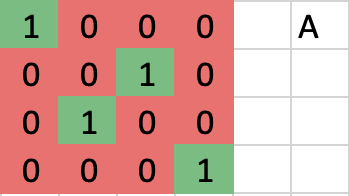
\includegraphics[scale=.5]{magic-squares/1.png}
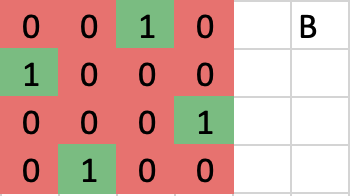
\includegraphics[scale=.5]{magic-squares/2.png}
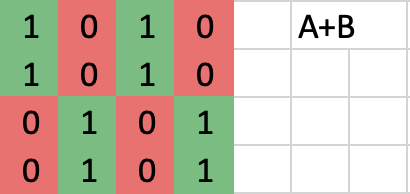
\includegraphics[scale=.5]{magic-squares/3.png}
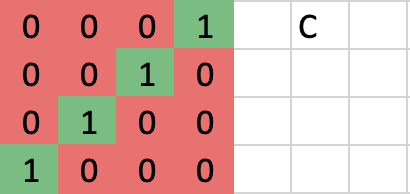
\includegraphics[scale=.5]{magic-squares/4.png}
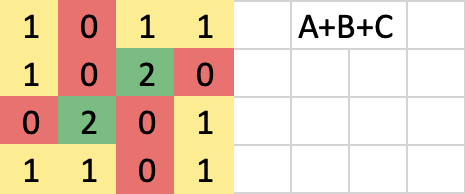
\includegraphics[scale=.5]{magic-squares/5.png}
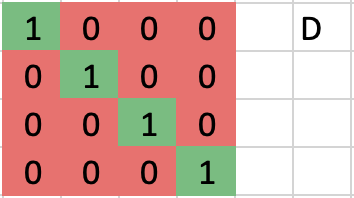
\includegraphics[scale=.5]{magic-squares/6.png}
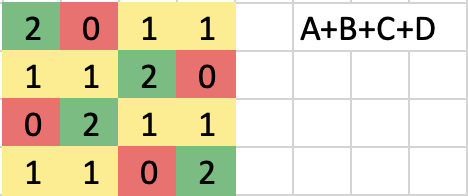
\includegraphics[scale=.5]{magic-squares/7.png}
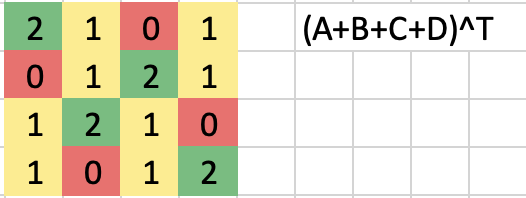
\includegraphics[scale=.5]{magic-squares/8.png}
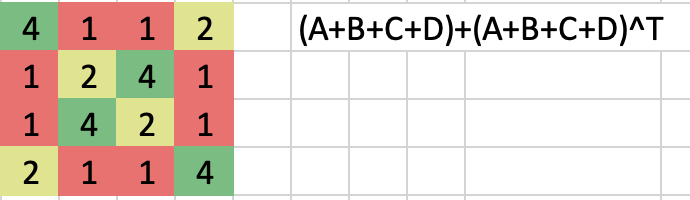
\includegraphics[scale=.5]{magic-squares/9.png}
\[
	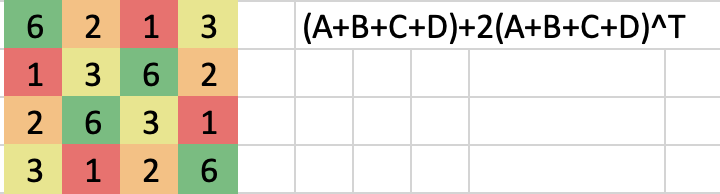
\includegraphics[scale=.5]{magic-squares/10.png}	
\]


\end{proof}

\end{document}